% !TeX spellcheck = en_GB
% !TeX encoding = UTF-8
\documentclass[8pt]{beamer}

/home/tobias/kesmaths-beamer/tex/preamble.tex

\usepackage{colortbl}

\usetikzlibrary{intersections}

\title[Discrete]{{\color{aa}\Huge\adfbullet{9}}AL FM Discrete}
\subtitle{Linear Programming: Simplex Algorithm, \textattachfile{LinearProgrammingSimplexAlgorithm.tex}{(TeX)}}

\begin{document}

\setlength{\abovedisplayskip}{0pt}
\setlength{\belowdisplayskip}{0pt}
\setlength{\abovedisplayshortskip}{0pt}
\setlength{\belowdisplayshortskip}{0pt}


\frame{\titlepage}

\begin{frame}{Overview}
	We have already seen that when we have a linear programming problem with two variables
we can represent the feasible region on a 2D graph and then find the optimal solution (which
will usually occur at a corner of the feasible region).

In theory, we could develop this idea with more variables but the problem is that there
would need to be an axis for each variable and therefore the graph would no longer be 2D.

\begin{definition}
	Instead we use an algorithmic method which involves starting at a vertex of the feasible
region and then making improvements until we find an optimal solution.
\end{definition}
\centering
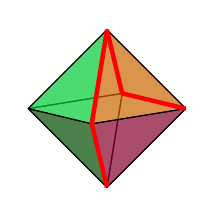
\begin{tikzpicture}[line join=bevel,z=-5.5]
\coordinate (A1) at (0,0,-1);
\coordinate (A2) at (-1,0,0);
\coordinate (A3) at (0,0,1);
\coordinate (A4) at (1,0,0);
\coordinate (B1) at (0,1,0);
\coordinate (C1) at (0,-1,0);

\draw (A1) -- (A2) -- (B1) -- cycle;
\draw (A4) -- (A1) -- (B1) -- cycle;
\draw (A1) -- (A2) -- (C1) -- cycle;
\draw (A4) -- (A1) -- (C1) -- cycle;
\draw [fill opacity=0.7,fill=green!80!blue] (A2) -- (A3) -- (B1) -- cycle;
\draw [fill opacity=0.7,fill=orange!80!black] (A3) -- (A4) -- (B1) -- cycle;
\draw [fill opacity=0.7,fill=green!30!black] (A2) -- (A3) -- (C1) -- cycle;
\draw [fill opacity=0.7,fill=purple!70!black] (A3) -- (A4) -- (C1) -- cycle;
\draw[color=red,ultra thick,yshift=0.01cm,xshift=0.01cm] (C1) -- (A3) -- (B1) -- (A1) -- (A4);
\end{tikzpicture}
\end{frame}

\begin{frame}[shrink=10]{Simplex Algorithm: Slack Variables}
	To start with we shall apply the Simplex Algorithm to a 2D problem. You could solve this by
drawing a graph but you might also be asked to specifically use the Simplex Algorithm.

\begin{problem}
	\begin{flalign*}
		\text{Maximise} && I &= x+0.8y && \hspace{5cm} \\
		\text{subject to} && x+y &\leq 1000 && \\
				  && 2x+y &\leq 1500 && \\
				  & 3x+2y &\leq 2400 && 
	.\end{flalign*}

\end{problem}

\begin{definition}
	\textbf{Step 1;}

	Replace the inequalities with \emph{slack variables} in order to replace them with equalities.
\end{definition}

          \begin{flalign*}
		  \text{Maximise}   && &I &    &       &      &      &     &       && \hspace{5cm} \\
		  \text{where}      && &I &- x &- 0.8y &      &      &     &= 0    &&              \\
		  \text{subject to} && &  &x   &+ y    &+ s_1 &      &     &= 1000 &&              \\
				    && &  &2 x &+ y    &      &+ s_2 &     &= 1500 &&              \\
				    && &  &3 x &+ 2y   &      &      &+s_3 &= 2400 &&
			    .\end{flalign*}
The slack variables $ s_1,s_2,s_3 \geq 0$ in order to ensure that the $\leq$ inequalities are satisfied.

\alert{The AQA syllabus states that you will only be assessed on problems with  $\leq$ inequalities.}

\end{frame}

\begin{frame}{Simplex Algorithm: Simplex Tableau}
	\begin{definition}
		\textbf{Step 2;}

		Find an initial solution (often when everything is zero) to create a simplex tableau.
	\end{definition}

	\begin{center}
\colorbox{cc!30}{
\begin{nicetable}{c|ccccc|c}
$I$ & $x$ & $y$ & $s_1$ & $s_2$ & $s_3$ & RHS \\ 
  \hline
1 & $-1$ & $-0.8$  & 0 & 0 & 0 & \tikzmarknode{A}{$0$}   \\ 
   \hline
0 & 1 & $1$  & 1 & 0 & 0 & 1000 \\ 
  0 & 2 & $1$  & 0 & 1 & 0 & 1500  \\ 
  0 & 3 & $2$  & 0 & 0 & 1 & 2400 \\ 
\end{nicetable}}
\end{center}

This is for the initial solution; $I=0,x=0,y=0,s_1 =1000, \tikzmarknode{B}{s_2=1500},s_3=2400$.

				\adjustbox{max width=.3\linewidth}{
					\begin{tikzpicture}[remember picture]
					\begin{axis}[mlineplot,width=5cm,height=5cm,
						xmin= -200, xmax= 1200,
						ymin= -200, ymax = 1600,
						axis lines = middle,
						xlabel={$x$},
						ylabel={$y$},
					]
					\addplot[color=aa,domain=-200:1200] {-x+1000};
					\addplot[color=aa,domain=-200:1200] {-2*x+1500};
					\addplot[color=aa,domain=-200:1200] {-6*x/4+4800/4};
					\fill[color=aa] (axis cs:0,0) circle[radius=4pt];
					\node (C) at (axis cs:0,0) {};
					\end{axis}
				\end{tikzpicture}
			}

\alert{It is not necessary to draw the graph but I include
here to give a picture of what is going on.}



\begin{tikzpicture}[overlay, remember picture]
	\draw[color=aa,<-] (A) --++ (0.5,0) node[right] {\sol[2]{\parbox{3cm}{Note we have reformulated the objective function from $I=x+0.8y$ to  $I-x-0.8y=0$}}};
	\draw[color=aa,<-] (B) --++ (0,-0.5) node[below,xshift=-1cm] {\sol[3]{\parbox{7cm}{The $s_1,s_2,s_3$ are how much 'slack' we have in each of the constraints. We are going to use this slack to increase the value of the objective function.}}};
	\draw[color=aa,<-] (C) --++ (0.3,-0.5) node[right] {\tiny Initial solution};
\end{tikzpicture}


\end{frame}


\begin{frame}[shrink=20]{Simplex Algorithm: Tableau Interpretation}

\begin{columns}
	\begin{column}{.6\linewidth}
	\begin{center}
\colorbox{cc!30}{
\begin{nicetable}{c|ccccc|c}
$I$ & $x$ & $y$ & $s_1$ & $s_2$ & $s_3$ & RHS \\ 
  \hline
1 & $-1$ & $-0.8$  & 0 & 0 & 0 & $0$   \\ 
   \hline
0 & 1 & $1$  & 1 & 0 & 0 & 1000 \\ 
  0 & 2 & $1$  & 0 & 1 & 0 & 1500  \\ 
  0 & \tikzmarknode{A}{3} & \tikzmarknode{B}{$2$}  & \tikzmarknode{C}{0} & \tikzmarknode{D}{0} & \tikzmarknode{E}{1} & 2400 \\ 
\end{nicetable}}
\end{center}
\end{column}
\begin{column}{.3\linewidth}
\begin{definition}
	At each stage of the algorithm the current values of the basic variables is the values on the right-hand side and the free variables \textbf{have value 0}. 
\end{definition}
\alert{This is important as it allows you to read off the current solution and each point and, when you get to Step 7, the final solution.}
\end{column}
\end{columns}

In our initial solution $ s_1,s_2$ and $s_3$ are basic which means we have used up as much of them as possible. $x$ and  $y$ are free meaning we are not using any of them and can potentially use some more.


So we can see that the initial solution is $I=0,x=0,y=0,s_1 =1000, \tikzmarknode{F}{s_2=1500},s_3=2400$.

				\adjustbox{max width=.3\linewidth}{
					\begin{tikzpicture}[remember picture]
					\begin{axis}[mlineplot,width=5cm,height=5cm,
						xmin= -200, xmax= 1200,
						ymin= -200, ymax = 1600,
						axis lines = middle,
						xlabel={$x$},
						ylabel={$y$},
					]
					\addplot[color=aa,domain=-200:1200] {-x+1000};
					\addplot[color=aa,domain=-200:1200] {-2*x+1500};
					\addplot[color=aa,domain=-200:1200] {-6*x/4+4800/4};
					\fill[color=aa] (axis cs:0,0) circle[radius=4pt];
					\node (G) at (axis cs:0,0) {};
					\end{axis}
				\end{tikzpicture}
			}

\alert{It is not necessary to draw the graph but I include
here to give a picture of what is going on.}



\begin{tikzpicture}[overlay, remember picture]
	\node[yshift=-0.5cm,xshift=-1cm,below,fill=cc,draw=aa] (H) at (A) {\parbox{5cm}{
	The variables correspond to the other columns and are called non-basic or free.
}};
	\draw[color=aa,->] (H) to (A);
	\draw[color=aa,->] (H) to (B);
	\node[yshift=-0.2cm,xshift=1.5cm,below,fill=cc,draw=aa] (I) at (E) {\parbox{4cm}{
	The variables which make up the identity matrix in the constraint rows are called basic variables.
	}};
\draw[color=aa,->] (I) to (C);
\draw[color=aa,->] (I) to (D);
\draw[color=aa,->] (I) to (E);
	\draw[color=aa,<-] (F) --++ (0,-0.5) node[below,xshift=-1cm] {\sol[3]{\parbox{7cm}{We are going to increase the objective function by using up as much of the $x$ and  $y$ as possible and less of the slack variables $s_1,s_2,s_3$.}}};
	\draw[color=aa,<-] (G) --++ (0.3,-0.5) node[right] {\tiny Initial solution};
\end{tikzpicture}


\end{frame}

\begin{frame}[shrink=10]{Simplex Algorithm: Find the Pivot Element}
	\begin{definition}
		\textbf{Step 3;} 

		The pivot column is the one with the most negative entry in the objective row.
	\end{definition}

\begin{center}
  \colorbox{cc!30}{
	  \begin{nicetable}{c|ccccc|c}
		  $I$ & \cellcolor{aa!50} $x$ & $y$ & $s_1$ & $s_2$ & $s_3$ & RHS \\ 
  \hline
  1 & \cellcolor{aa!50} $-1$ & $-0.8$  & 0 & 0 & 0 & $0$   \\ 
    \hline
  0 & \cellcolor{aa!50} 1 & $1$  & 1 & 0 & 0 & 1000 \\ 
    0 & \cellcolor{aa!50} 2 & $1$  & 0 & 1 & 0 & 1500  \\ 
    0 & \cellcolor{aa!50} 3 & $2$  & 0 & 0 & 1 & 2400 \\ 
  \end{nicetable}}
  \end{center}

	\begin{definition}
		\textbf{Step 4;} 
The pivot element is the entry in the pivot column with smallest \textbf{positive} value for $\frac{\text{RHS}}{\text{variable}}$.
	\end{definition}


\begin{center}
  \colorbox{cc!30}{
	  \begin{nicetable}{c|ccccc|c|c}
		  $I$ & \cellcolor{aa!50} $x$ & $y$ & $s_1$ & $s_2$ & $s_3$ & RHS & $\frac{\text{RHS}}{x}$ \\ 
  \hline
		  1 & \cellcolor{aa!50} $-1$ & $-0.8$  & 0 & 0 & 0 & $0$  & \\ 
    \hline
		  0 & \cellcolor{aa!50} 1 & $1$  & 1 & 0 & 0 & 1000 & $\frac{1000}{1}=1000$\\ 
		  0 & \cellcolor{red} 2 & $1$  & 0 & 1 & 0 & 1500 & $\frac{1500}{2}=\tikzmarknode{A}{750} $ \\ 
		  0 & \cellcolor{aa!50} 3 & $2$  & 0 & 0 & 1 & 2400 & $\frac{2400}{3}=800$ \\ 
  \end{nicetable}}
  \end{center}
	
  \alert{The reason we choose the minimum is that this is the limiting constraint. This will make more sense on the next slide.}

  \begin{tikzpicture}[overlay, remember picture]
	  \draw[color=aa,<-] (A) --++ (0.5,0) node[right,scale=0.6,fill=cc,draw=aa] {\parbox{4cm}{750 is the smallest positive value so the pivot is the element in this row in the pivot column.}};
  \end{tikzpicture}
\end{frame}



\begin{frame}{Simplex Algorithm: Pivoting}
	\begin{definition}
		\textbf{Step 5;} 
Divide everything in the pivot row by the pivot element.
	\end{definition}

\begin{center}
  \colorbox{cc!30}{
	  \begin{nicetable}{c|ccccc|c}
		  $I$ &$x$ & $y$ & $s_1$ & $s_2$ & $s_3$ & RHS \\ 
  \hline
  1 & $-1$ & $-0.8$  & 0 & 0 & 0 & $0$   \\ 
    \hline
  0 & 1 & $1$  & 1 & 0 & 0 & 1000 \\ 
    0 & 1 & $0.5$  & 0 & 0.5 & 0 & 750  \\ 
    0 & 3 & $2$  & 0 & 0 & 1 & 2400 \\ 
  \end{nicetable}}
  \end{center}

	\begin{definition}
		\textbf{Step 6;} 
		Do row operations to make everything all the other elements in the pivot column zero.
	\end{definition}


  \colorbox{cc!30}{
	  \begin{nicetable}{c|ccccc|c}
		  $I$ & $x$ & $y$ & $s_1$ & $s_2$ & $s_3$ & RHS  \\ 
  \hline
		  1 & $0$ & $-0.3$  & 0 & 0.5 & 0 & \tikzmarknode{A}{$750$}   \\ 
    \hline
		  0 &  0 & $0.5$  & 1 & $-0.5$ & 0 & \tikzmarknode{B}{250} \\ 
		  0 &  1 & $0.5$  & 0 & $0.5$ & 0 & 750  \\ 
		  0 &  0 & $0.5$  & 0 & $-1.5$ & 1 & \tikzmarknode{C}{150}  \\ 
  \end{nicetable}}
	

  \begin{tikzpicture}[overlay, remember picture]
	  \draw[color=aa,<-] (A) --++ (0.5,0) node[right,scale=0.6,fill=cc,draw=aa] {Objective Row $+$ Pivot Row in table above.};
	  \draw[color=aa,<-] (B) --++ (0.5,0) node[right,scale=0.6,fill=cc,draw=aa] {First Constraint Row $-$ Pivot Row in table above.};
	  \draw[color=aa,<-] (C) --++ (0.5,0) node[right,scale=0.6,fill=cc,draw=aa] {Third Constraint Row $-3 \times $ Pivot Row in table above.};
  \end{tikzpicture}
\end{frame}

 \begin{frame}{Simplex Algorithm: Pivoting Interpretation}
  
  
    \colorbox{cc!30}{
            \begin{nicetable}{c|ccccc|c}
                    $I$ & $x$ & $y$ & $s_1$ & $s_2$ & $s_3$ & RHS  \\
    \hline
                    1 & $0$ & $-0.3$  & 0 & 0.5 & 0 & $750$ \\
      \hline
                    0 &  0 & $0.5$  & 1 & $-0.5$ & 0 & 250 \\
                    0 &  1 & $0.5$  & 0 & $0.5$ & 0 & 750  \\
                    0 &  0 & $0.5$  & 0 & $-1.5$ & 1 & 150  \\
    \end{nicetable}}
  
  In our latest tableau we can see that $x$, $ s_1$ and $ s_3$ are basic and $y$ and $ s_2$ are free. Therefore in our current situation we are using up as much of $x, s_1$ and $s_3$ as possible and none of $y$ and $ s_2$.
  
  \begin{definition}
  Pivoting will make one free variable basic and one basic variable free.
  \end{definition}

So our current solution is $I=750,x=750,y=0,s_1 =0, s_3=150$.

\begin{columns}
\begin{column}{.5\linewidth}
				\adjustbox{max width=.6\linewidth}{
					\begin{tikzpicture}[remember picture]
					\begin{axis}[mlineplot,width=5cm,height=5cm,
						xmin= -200, xmax= 1200,
						ymin= -200, ymax = 1600,
						axis lines = middle,
						xlabel={$x$},
						ylabel={$y$},
					]
					\addplot[color=aa,domain=-200:1200] {-x+1000};
					\addplot[color=aa,domain=-200:1200] {-2*x+1500};
					\addplot[color=aa,domain=-200:1200] {-6*x/4+4800/4};
					\fill[color=aa] (axis cs:750,0) circle[radius=4pt];
					\node (G) at (axis cs:750,0) {};
					\end{axis}
				\end{tikzpicture}
			}

\end{column}
\begin{column}{.5\linewidth}
So what has happened on this pivot is
we’ve used as much $x$ as we can and
we had to stop at the green line
which was the second constraint
(which was indicated to us by having
the lowest ratio).
\end{column}
\end{columns}

\begin{tikzpicture}[overlay, remember picture]
	\draw[color=aa,<-] (G) --++ (0.3,-0.5) node[right] {\tiny Current solution};
\end{tikzpicture}
\end{frame}

\begin{frame}{Simplex Algorithm: Pivoting Again}
	\begin{definition}
		\textbf{Step 7;}

	Repeat until everything in the objective row is non-negative. 
	\adjustbox{max width=.25\linewidth}{\begin{minipage}{.4\linewidth} \alert{Note it says \emph{non-negative} which is different to positive (because 0 is non-negative).} \end{minipage}}
	\end{definition}
	
\begin{center}
  \colorbox{cc!30}{
	  \begin{nicetable}{c|ccccc|c|c}
		  $I$ & $x$ &  \cellcolor{aa!50} $y$    & $s_1$ & $s_2$  & $s_3$ & RHS & $\frac{\text{RHS}}{x}$ \\ \hline
		  1 &   $0$ &  \cellcolor{aa!50} $-0.3$ & 0     & $0.5$  & 0 & $750$  & \\ \hline
\tikzmarknode{B}{0} &     0 &  \cellcolor{aa!50} $0.5$  & 1     & $-0.5$ & 0 & 250 & $\frac{250}{0.5}=500$\\ 
		  0 &     1 &  \cellcolor{aa!50} $0.5$  & 0     & $0.5$  & 0 & 750 & $\frac{750}{0.5}=\tikzmarknode{A}{1500} $ \\ 
		  0 &     0 &  \cellcolor{red}   $0.5$  & 0     & $-1.5$ & 1 & 150 & $\frac{150}{0.5}=300$ \\ 
  \end{nicetable}}
  \end{center}


\begin{columns}
\begin{column}{.5\linewidth}
	\adjustbox{max width=\linewidth}{
  \colorbox{cc!30}{
	  \begin{nicetable}{c|ccccc|c}
		  \tikzmarknode{C}{$I$} & $x$ & $y$    & $s_1$ & $s_2$  & $s_3$ & RHS \\ \hline
		  1 &   $0$ & $-0.3$ & 0     & $0.5$  & 0 & \tikzmarknode{D}{$750$}   \\ \hline
                  0 &     0 & $0.5$  & 1     & $-0.5$ & 0 & 250     \\ 
		  0 &     1 & $0.5$  & 0     & $0.5$  & 0 & 750     \\ 
		  0 &     0 & $1$    & 0     & $-3$   & 2 & 300     \\ 
  \end{nicetable}}
  }
\end{column}
\begin{column}{.5\linewidth}
	\adjustbox{max width=\linewidth}{
  \colorbox{cc!30}{
	  \begin{nicetable}{c|ccccc|c}
		  $I$ & $x$ & $y$    & $s_1$ & $s_2$   & $s_3$ & RHS \\ \hline
\tikzmarknode{E}{1} &   $0$ & $0$    & 0     & $-0.4$  & $0.6$ & $840$   \\ \hline
                  0 &     0 & $0$    & 1     & $1$     & $-1$ & 100     \\ 
		  0 &     1 & $0$    & 0     & $2$     & $-1$ & 600     \\ 
		  0 &     0 & $1$    & 0     & $-3$    & 2    & 300     \\ 
  \end{nicetable}}
  }

\end{column}
\end{columns}

\begin{tikzpicture}[overlay,remember picture]
	\draw[color=aa,->] (B) -- node[midway, anchor=south east, align=left,scale=0.5] {Divide the pivot \\ row by 0.5} (C);
	\node[align=left,right,xshift=0.5cm,scale=0.5] at (A) {This time $y$ \\ is the pivot \\ column};
	\draw[color=aa,->] ($(D)+(-0.5,0)$) -- node[midway, below, align=left,scale=0.5] {Row operations \\ to make other \\ entries in pivot \\ column zero } (E.west);
\end{tikzpicture}


\end{frame}

 \begin{frame}{Simplex Algorithm: Second Pivot Interpretation}
  
  	  \begin{nicetable}{c|ccccc|c}
		  $I$ & $x$ & $y$    & $s_1$ & $s_2$   & $s_3$ & RHS \\ \hline
		  1 &   $0$ & $0$    & 0     & $-0.4$  & $0.6$ & $840$   \\ \hline
                  0 &     0 & $0$    & 1     & $1$     & $-1$ & 100     \\ 
		  0 &     1 & $0$    & 0     & $2$     & $-1$ & 600     \\ 
		  0 &     0 & $1$    & 0     & $-3$    & 2    & 300     \\ 
  \end{nicetable}
  
The basic variables are now $x,y$ and $ s_1$ and the free variables are $ s_2$ and $ s_3$.


So our current solution is $I=840,x=600,y=300,s_1 =100, s_2=0, s_3=0$.

\begin{columns}
\begin{column}{.5\linewidth}
				\adjustbox{max width=.6\linewidth}{
					\begin{tikzpicture}[remember picture]
					\begin{axis}[mlineplot,width=5cm,height=5cm,
						xmin= -200, xmax= 1200,
						ymin= -200, ymax = 1600,
						axis lines = middle,
						xlabel={$x$},
						ylabel={$y$},
					]
					\addplot[color=aa,domain=-200:1200] {-x+1000};
					\addplot[color=aa,domain=-200:1200] {-2*x+1500};
					\addplot[color=aa,domain=-200:1200] {-6*x/4+4800/4};
					\fill[color=aa] (axis cs:600,300) circle[radius=4pt];
					\node (G) at (axis cs:600,300) {};
					\end{axis}
				\end{tikzpicture}
			}

\end{column}
\begin{column}{.5\linewidth}
	Because there is still a negative entry
	in the objective row our solution is not yet optimal and we must continue...
\end{column}
\end{columns}

\begin{tikzpicture}[overlay, remember picture]
	\draw[color=aa,<-] (G) --++ (0.3,-0.5) node[right] {\tiny Current solution};
\end{tikzpicture}
\end{frame}

\begin{frame}{Simplex Algorithm: Pivoting Again}
	
\begin{center}
  \colorbox{cc!30}{
	  \begin{nicetable}{c|ccccc|c|c}
		  $I$ & $x$ & $y$  & $s_1$ & \cellcolor{aa!50}$s_2$  & $s_3$ & RHS & $\frac{\text{RHS}}{s_2}$  \\ \hline
		  1 &   $0$ & $0$  & 0     & \cellcolor{aa!50}$-0.4$ & $0.6$ & 840 &                         \\ \hline
		  0 &     0 & $0$  & 1     & \cellcolor{red}   $1$   & $-1$  & 100 & $\frac{100}{1}=100$   \\ 
		  0 &     1 & $0$  & 0     & \cellcolor{aa!50}$2$    & $-1$  & 600 & $\frac{600}{2}=300 $ \\ 
		  0 &     \tikzmarknode{B}{0} & $1$  & 0     & \cellcolor{aa!50}$-3$   & $2$   & 300 & \tikzmarknode{A}{$\frac{300}{-3}=-100$}   \\ 
  \end{nicetable}}
  \end{center}


\begin{columns}
\begin{column}{.5\linewidth}
	\adjustbox{max width=\linewidth}{
  \colorbox{cc!30}{
	  \begin{nicetable}{c|ccccc|c}
		  \tikzmarknode{C}{$I$} & $x$ & $y$    & $s_1$ & $s_2$  & $s_3$ & RHS \\ \hline
		  1 &   $0$ & $0$ & 0     & $-0.4$ & $0.6$ & \tikzmarknode{D}{$840$}   \\ \hline
                  0 &     0 & $0$ & 1     & $1$    & $-1$ & 100     \\ 
		  0 &     1 & $0$ & 0     & $2$    & $-1$ & 600     \\ 
		  0 &     0 & $1$ & 0     & $-3$   & 2 & 300     \\ 
  \end{nicetable}}
  }
\end{column}
\begin{column}{.5\linewidth}
	\adjustbox{max width=\linewidth}{
  \colorbox{cc!30}{
	  \begin{nicetable}{c|ccccc|c}
		  $I$ & $x$ & $y$    & $s_1$ & $s_2$   & $s_3$ & RHS \\ \hline
\tikzmarknode{E}{1} &   $0$ & $0$    & $0.4$ & $0$  & $0.2$ & $880$   \\ \hline
                  0 &     0 & $0$    & 1     & $1$  & $-1$  & 100     \\ 
		  0 &     1 & $0$    & $-2$  & $0$  & $1$   & 400     \\ 
		  0 &     0 & $1$    & 3     & $0$  & $-1$  & 600     \\ 
  \end{nicetable}}
  }

\end{column}
\end{columns}

\begin{tikzpicture}[overlay,remember picture]
	\draw[color=aa,->] (B) -- node[midway, anchor=south east, align=left,scale=0.5] {Here the pivot element is 1 so dividing \\ by it leaves the row unchanged.} (C);
	\node[align=left,right,xshift=1.5cm,scale=0.5] at (A) {Remember we are \\ looking for the smallest \\ positive value.};
	\draw[color=aa,->] (D) -- node[midway, below, align=left,scale=0.5] {Row operations \\ to make other \\ entries in pivot \\ column zero. } (E.west);
\end{tikzpicture}


\end{frame}


\begin{frame}{Past Paper Question}
	A company repairs and sells computer hardware, including monitors, hard drives and keyboards.

	Each monitor takes 3 hours to repair and the cost of components is 40 pounds.

	Each hard drive takes 2 hours to repair and the cost of components is 20 pounds.

	Each keyboard takes 1 hour to repair and the cost of components is 5 pounds.

	Each month, the business has 360 hours available for repairs and 2500 pounds available to buy components.

	Each month, the company sells all of its repaired hardware to a local computer shop.

	Each monitor, hard drive and keyboard sold gives the company a profit of 80, 35 and 15 pounds respectively.

	The company repairs and sells $x$ monitors, $y$ hard drives and $z$ keyboards each month.

	The company wishes to maximise its total profit.

	\begin{problem}
		\begin{itemize}
			\item Find five inequalities involving $x,y$ and $z$ for the company's problem.
			\item Find how many of each type of computer hardware the company should repair and sell each month.
			\item Explain how you know that you had reached the optimal solution.
			\item The local computer shop complains that they are not receiving one of the types of computer hardware that the company repairs and sells.

				Using the previous answer, suggest a way in which the company's problem can be modified to address the complaint.
		\end{itemize}
	\end{problem}
\end{frame}

\begin{frame}{Past Paper Solution}
	\begin{columns}[T]
		\begin{column}{.3\linewidth}
	\begin{solution}<2->
		$3x+2y+z \leq 360$ 

		$40x+20y+5z \leq 2500$ 

		$x \geq 0, y \geq 0, z \geq 0$.
	\end{solution}
	\begin{solution}<4->
		The objective row of the final tableau being non-negative numbers.
	\end{solution}
	\begin{solution}<5->
		As $y=0$, enforce some hard drives to be repaired by requiring that, for instance, $y \geq 10$.
	\end{solution}
\end{column}
\begin{column}{.7\linewidth}
	\begin{solution}<3->
		\centering
		\colorbox{cc!30}{
			\begin{nicetable}{c|ccccc|c}
				$P$ &  $x$  & $y$   & $z$   & $s$   & $t$   & value \\ \hline
				1   & $-80$ & $-35$ & $-15$ & 0     & 0     & 0     \\
				0   & 3     & 2     & 1     & 1     & 0     & 360   \\
				0   & \cellcolor{red} 40 & 20 & 5 & 0 & 1 & 2500    \\ \hline
				1   & 0     & 5     & $-5$  & 0     & 2     & 5000  \\
				0   & 0     & 0.5 & \cellcolor{red} 0.625 & 1 & $-0.075$ & 172.5 \\
				0 & 1 & 0.5 & 0.125 & 0 & 0.025 & 62.5 \\ \hline
				1 & 0 & 9 & 0 & 8 & 1.4 & 6380 \\
				0 & 0 & 0.8 & 1 & 1.6 & $-0.12$ & 276 \\
				0 & 1 & 0.4 & 0 &  $-0.2$ & 0.04 & 28 \\

			\end{nicetable}
		}

	To maximise profit the company should repair and sell 28 monitors, 0 hard drives and 276 keyboards each month.
	\end{solution}
\end{column}
\end{columns}
\end{frame}


\end{document}

